\chapter{Membangun Model Prediksi}
\section{Teori}

\subsection{Binary Classification}

\par Setiap data dalam klasifikasi biner memiliki atribut kelas yang berisi dua nilai. Nilai suatu kelas dapat dinyatakan sebagai positif atau negatif. 0 atau 1; benar atau salah; dll. Contoh klasifikasi biner: pemfilteran spam (model klasifikasi yang mendeteksi apakah email diklasifikasikan sebagai spam atau non-spam).\cite{binary}

\begin{figure}[H]
    \centering
    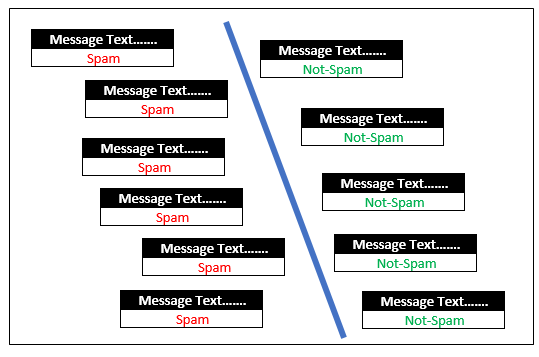
\includegraphics[width=12cm]{figures/chapter2/1.png}
    \caption{Contoh Spam Filtering, Garis Miring Biru adalah class boundary}
\end{figure}

\subsection{Supervised Learning, Unsupervised Learning, dan Clustering}

\par Supervised Learning biasanya digunakan untuk menyelesaikan masalah klasifikasi dan regresi. Algoritma sangat bergantung pada penerapan input dan output pada kumpulan data tertentu, jadi kami (pengguna / ilmuwan data) memainkan peran utama dalam memverifikasi input dan output ini. Perhatikan gambar berikut.

\begin{figure}[H]
    \centering
    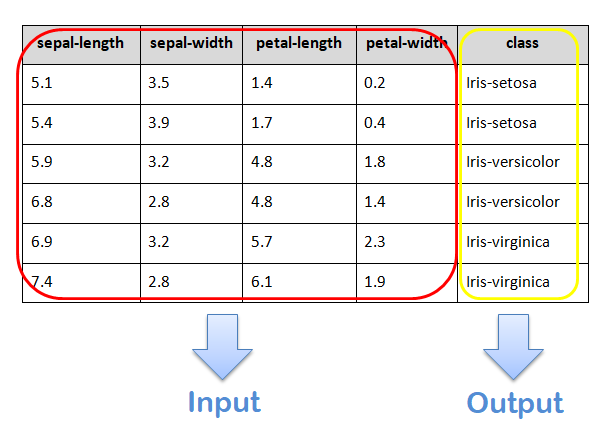
\includegraphics[width=12cm]{figures/chapter2/2.png}
    \caption{Supervised Learning: Dataset Iris}
\end{figure}

\par Pada gambar di atas, input merupakan variabel yang akan diamati, lalu output adalah hasilnya. Dataset iris telah memiliki kategori yang menjadi class, jika kita memasukkan input baru akan keluar hasil sesuai dengan kategori, pada contoh di atas keluar kategori iris-setosa.

\par Unsupervised Learning berarti tidak mengawasi dan memandu model machine learning, tetapi membiarkan model tersebut belajar dengan sendirinya untuk menemukan informasi yang mungkin tidak terlihat oleh mata manusia. Perhatikan gambar berikut.

\begin{figure}[H]
    \centering
    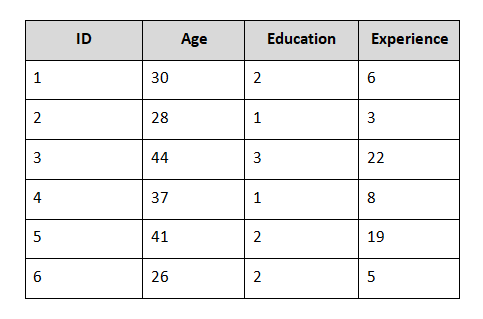
\includegraphics[width=12cm]{figures/chapter2/3.png}
    \caption{Unsupervised Learning}
\end{figure}

\par Seperti yang dapat dilihat dari contoh data di atas, data yang diberikan hanya berupa variabel masukan, tanpa label (Output). Dalam hal ini, model berlatih pada kumpulan data, kemudian mencari informasi dan menarik kesimpulannya sendiri dari data tersebut.

\par Clustering atau pengelompokan merupakan salah satu masalah dalam penggunaan teknik unsupervised learning. Contoh cluster termasuk segmentasi perbankan pelanggan atau segmentasi berita online.

\par Pada dasarnya, jika kumpulan data tidak memiliki label class, teknik unsupervised learning akan digunakan. Dengan kata lain, algoritma dapat secara otomatis membagi data menjadi beberapa cluster berdasarkan kriteria tertentu (seperti kesamaan).\cite{learning}

\subsection{Evaluasi dan Akurasi}

\begin{figure}[H]
    \centering
    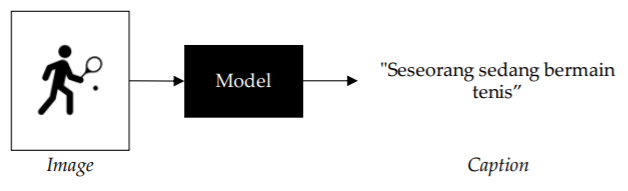
\includegraphics[width=12cm]{figures/chapter2/4.PNG}
    \caption{Model Evaluasi}
\end{figure}

\par Pada gambar di atas, bagaimana Anda mengevaluasi apakah model dapat memberikan penjelasan yang mencerminkan situasi gambar? Misalnya, jika gambar diberikan "Seseorang sedang bermain tenis" dan model memprediksi "Seseorang bermain bola basket", model memberikan interpretasi yang salah. Namun, jika Anda melihat proporsi dari jumlah kata yang sama, Anda berharap ada banyak kata di output yang cocok dengan prediksi, yaitu "seseorang sedang bermain".\cite{evaaku}

\par Akurasi adalah indikator kinerja paling sederhana dan sering digunakan saat mengevaluasi kinerja model. Akurasi didefinisikan sebagai proporsi prediksi yang benar dibagi dengan jumlah sampel. Mengingat output yang diperlukan (juga dikenal sebagai "gold standard") y dan hasil prediksi ˆy, dengan menghitung rasio jumlah elemen yang sama antara y dan ˆy. Secara matematis akurasi dirumuskan dengan persamaan, dimana N merepresentasikan jumlah sampel.\cite{evaaku}

\begin{figure}[H]
    \centering
    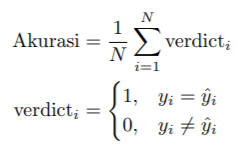
\includegraphics[width=12cm]{figures/chapter2/5.PNG}
    \caption{Akurasi}
\end{figure}

\subsection{Confusion Matrix}

\par Confusion Matrix juga biasa disebut sebagai Error Matrix. Pada dasarnya, confusion matrix memberikan informasi tentang perbandingan hasil klasifikasi yang dilakukan oleh sistem (model) dengan hasil klasifikasi yang sebenarnya. Matriks konfusi berbentuk tabel matriks yang mendeskripsikan performa model klasifikasi pada rangkaian data uji dengan nilai sebenarnya yang diketahui. Gambar di bawah ini adalah matriks konfusi, yang berisi 4 kombinasi berbeda dari nilai prediksi dan nilai aktual. Lihatlah gambar di bawah ini:\cite{matrix}

\begin{figure}[H]
    \centering
    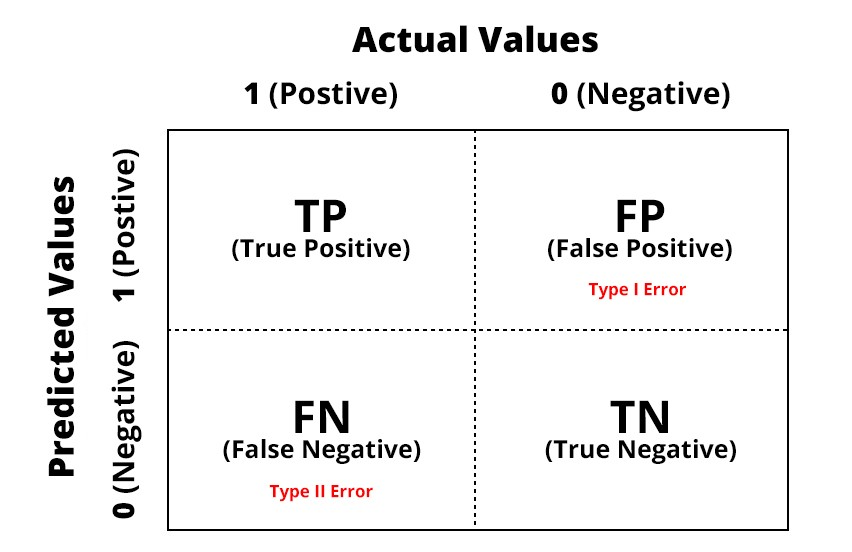
\includegraphics[width=12cm]{figures/chapter2/6.jpeg}
    \caption{Confusion Matrix}
\end{figure}

\begin{itemize}
    \item True Positive (TP)
    \par Ini adalah data positif yang prediksinya benar. Misalnya, pasien menderita kanker (tingkat 1), dan model memprediksi bahwa pasien menderita kanker (tingkat 1).
    \item True Negative (TN)
    \par Menunjukkan data negatif yang diperkirakan benar. Misalnya, pasien tidak mengidap kanker (level 2), dan model memprediksi bahwa pasien tidak mengidap kanker (level 2).
    \item False Postive (FP) — Type I Error
    \par Ini adalah angka negatif, tetapi ramalannya adalah angka positif. Misalnya pasien tidak menderita kanker (kategori 2), tetapi model yang memprediksi bahwa pasien tersebut menderita kanker (kategori 1).
    \item False Negative (FN) — Type II Error
    \par Ini adalah angka positif, tetapi ramalannya adalah angka negatif. Misalnya, seorang pasien mengidap kanker (grade 1), tetapi model memprediksi bahwa pasien tersebut tidak mengidap kanker (grade 2).
\end{itemize}

\subsection{K-Fold Cross Validation}

\par K-fold cross validation merupakan teknik verifikasi dalam pengembangan model verifikasi terpisah, dimana verifikasi mengukur training error dengan menggunakan data uji atau test data untuk pengujian. Pengembangan cross validation sendiri dikarenakan terdapat kelemahan pada model sebelumnya yaitu sampel dipilih secara random, sehingga test error sampling tidak dapat menetapkan kelas secara terstruktur. Walaupun hasil yang didapat dapat dimaksimalkan, tes yang lebih efektif tidak dapat dicapai. Kemudian muncul cross validation, yang dapat bekerja dengan cepat dengan pengambilan sampel yang lebih terstruktur. Oleh karena itu, meskipun dalam jumlah pengujian, data yang berbeda dari eksperimen atau literasi sebelumnya akan digunakan untuk mendapatkan beberapa training dataset dan testing dataset.\cite{cross}

\begin{figure}[H]
    \centering
    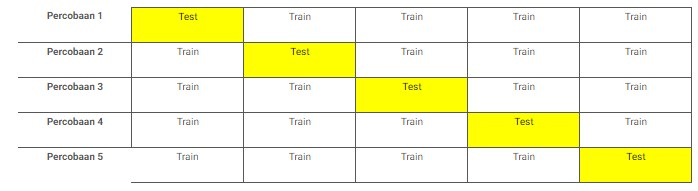
\includegraphics[width=12cm]{figures/chapter2/7.jpg}
    \caption{5-Fold Cross Validation}
\end{figure}

\par Percobaan di atas merupakan contoh validasi silang 5 kali lipat, yang artinya percobaan tersebut perlu dilakukan 5 tahap. Percobaan 1, untuk mengubah bagian pertama dari partisi menjadi data test, dan partisi lainnya menjadi data training, dan seterusnya. 

\par Dari 5 hasil percobaan ini, kita akan menggunakan confusion matrix untuk mencatat nilai evaluasi kinerja model, kemudian menentukan nilai rata-rata setiap percobaan. Kemudian, akan ditemukan eksperimen mana yang dapat digunakan sebagai referensi untuk menggunakan model algoritma yang dipilih.

\subsection{Decision Tree}

\begin{figure}[H]
    \centering
    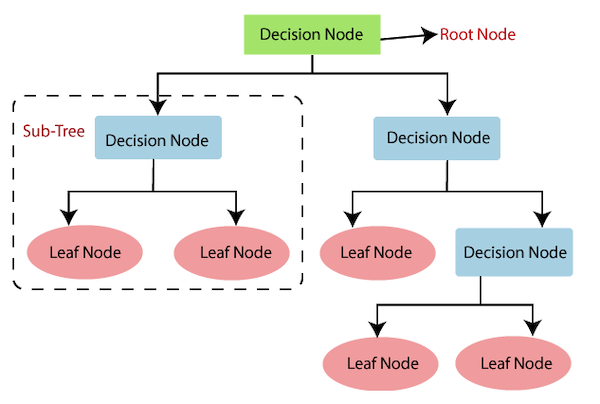
\includegraphics[width=12cm]{figures/chapter2/8.png}
    \caption{5-Fold Cross Validation}
\end{figure}

\par Decision Tree adalah diagram yang dapat membantu Anda memilih salah satu dari beberapa opsi pengoperasian. Biasanya, dimulai dengan satu atau lebih node. Kemudian, cabang node menunjukkan opsi yang tersedia. Selain itu, setiap cabang tersebut akan memiliki cabang baru. Oleh karena itu, cara ini dinamakan "Tree" karena mirip dengan pohon yang banyak cabangnya. Decision tree dapat membuat berbagai pilihan dan menyelidiki kemungkinan hasil dari pilihan tersebut. Selain itu, Anda juga dapat melihat potensi risiko dan keuntungan dari setiap opsi. Mengutip dari Venngage, decision tree mengandung tiga unsur, yaitu:\cite{tree}

\begin{itemize}
    \item Root Node (Akar): tujuan akhir atau keputusan besar yang harus dibuat.
    \item Branches (Ranting): berbagai opsi tindakan.
    \item Leaf Node (Daun): kemungkinan hasil atas setiap opsi tindakan.
\end{itemize}

\subsection{Entropi dan Information Gain}

\par Pohon keputusan dibangun dari simpul akar dari atas ke bawah dan melibatkan pembagian data menjadi subset yang berisi contoh nilai yang sama (homogen). Algoritma ID3 menggunakan entropi untuk menghitung keseragaman sampel. Jika sampel benar-benar seragam, entropinya nol; jika distribusi sampel sama, entropi adalah 1.\cite{entropi}

\begin{figure}[H]
    \centering
    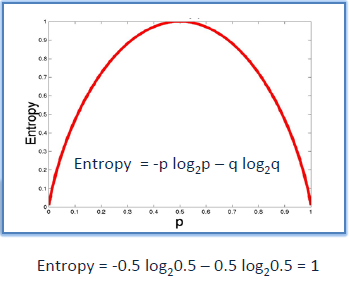
\includegraphics[width=12cm]{figures/chapter2/9.png}
    \caption{Entrophy}
\end{figure}

\begin{enumerate}
    \item Entropi yang menggunakan tabel frekuensi atribut tunggal:
    \begin{figure}[H]
        \centering
        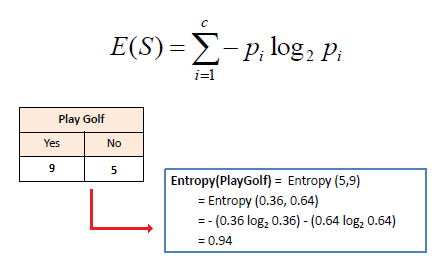
\includegraphics[width=12cm]{figures/chapter2/10.png}
        \caption{Entrophy Atribut Tunggal}
    \end{figure}
    \item Entropi yang menggunakan tabel frekuensi dua atribut:
    \begin{figure}[H]
        \centering
        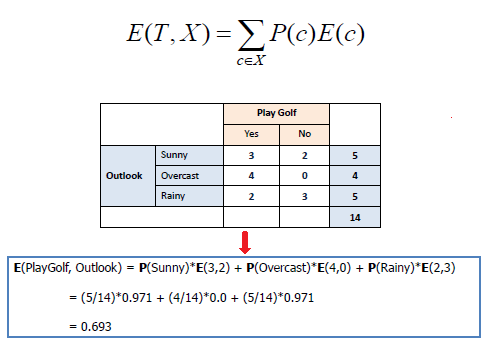
\includegraphics[width=12cm]{figures/chapter2/11.png}
        \caption{Entrophy Dua Atribut}
    \end{figure}
\end{enumerate}

\par Information gain didasarkan pada pengurangan entropi setelah kumpulan data dibagi dengan atribut. Keseluruhan proses membangun pohon keputusan adalah menemukan atribut yang mengembalikan perolehan informasi tertinggi (yaitu, cabang yang paling homogen).

\begin{enumerate}
    \item Langkah Pertama: Hitung Entropi.
    \begin{figure}[H]
        \centering
        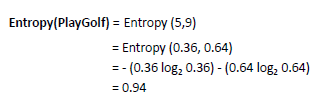
\includegraphics[width=12cm]{figures/chapter2/12.png}
        \caption{Langkah 1}
    \end{figure}
    \item Langkah 2: Kemudian bagi kumpulan data menjadi atribut yang berbeda. Hitung entropi setiap cabang. Kemudian tambahkan secara proporsional untuk mendapatkan nilai entropi dari pembagian tersebut. Kurangi entropi yang dihasilkan dari entropi sebelum pemisahan. Hasilnya adalah penurunan perolehan informasi atau entropi.
    \begin{figure}[H]
        \centering
        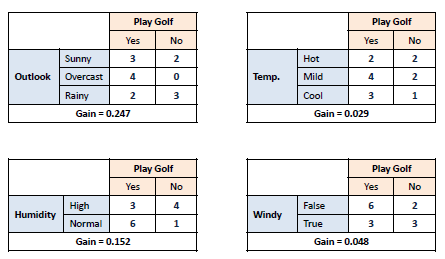
\includegraphics[width=12cm]{figures/chapter2/13.png}
    \end{figure}
    \begin{figure}[H]
        \centering
        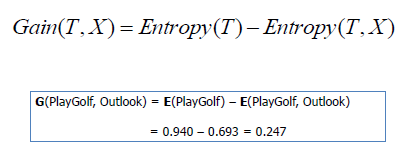
\includegraphics[width=12cm]{figures/chapter2/14.png}
        \caption{Langkah 2}
    \end{figure}
    \item Langkah 3: Pilih atribut dengan perolehan informasi terbesar sebagai simpul keputusan, bagi kumpulan data menjadi beberapa cabang, dan ulangi proses yang sama pada setiap cabang.
    \begin{figure}[H]
        \centering
        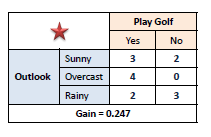
\includegraphics[width=12cm]{figures/chapter2/15.png}
    \end{figure}
    \begin{figure}[H]
        \centering
        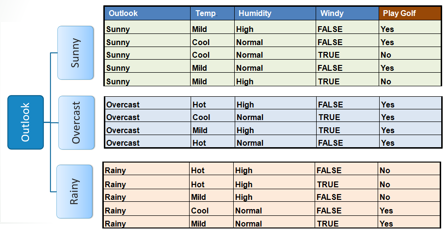
\includegraphics[width=12cm]{figures/chapter2/16.png}
        \caption{Langkah 3}
    \end{figure}
    \item Langkah 4a: Cabang dengan entropi 0 adalah simpul daun.
    \begin{figure}[H]
        \centering
        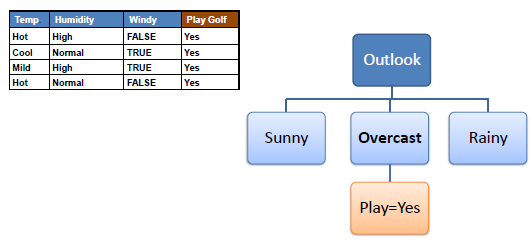
\includegraphics[width=12cm]{figures/chapter2/17.png}
        \caption{Langkah 4a}
    \end{figure}
    \item Langkah 4b: Cabang dengan entropi lebih besar dari 0 akan dipecah lagi.
    \begin{figure}[H]
        \centering
        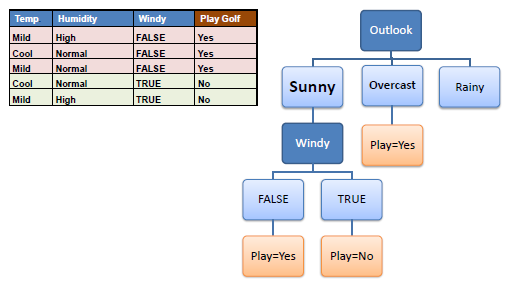
\includegraphics[width=12cm]{figures/chapter2/18.png}
        \caption{Langkah 4b}
    \end{figure}
\end{enumerate}

\section{Scikit Learn}

\par Dataset ambil di https://github.com/PacktPublishing/Python-Artificial-Intelligence-Projects-for-Beginners folder Chapter01. Tugas anda adalah, dataset ganti menggunakan student-mat.csv dan mengganti semua nama variabel dari kode di bawah ini dengan nama-nama makanan (NPM mod 3=0), kota (NPM mod 3=1), buah (NPMmod 3=2).

\subsection{Nomor 1}
\begin{lstlisting}[language=Python]
import pandas as pd #import library pandas dengan alias pd
akiba = pd.read_csv('D:/[Matkul]/AI/Chapter 2/Python-Artificial-Intelligence-Projects-for-Beginners-master/Chapter01/dataset/student-mat.csv', sep=';') #sebuah variable akiba untuk memanggil file csv
len(akiba) #untuk menghitung jumlah data di file csv
\end{lstlisting}

\par Hasilnya:

\begin{figure}[H]
    \centering
    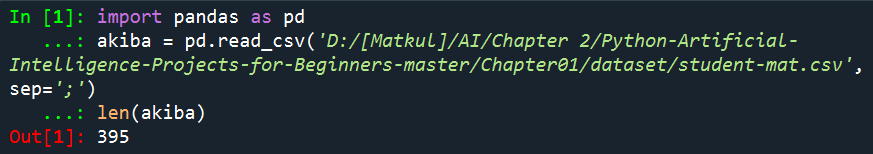
\includegraphics[width=12cm]{figures/chapter2/19.PNG}
    \caption{Nomor 1}
\end{figure}

\subsection{Nomor 2}

\begin{lstlisting}[language=Python]
akiba['pass'] = akiba.apply(lambda row: 1 if (row['G1']+row['G2']+row['G3'])>= 35 else 0, axis=1) #membuat label binary pass atau fail berdasarkan G1G2G3 dengan batas data lebih atau sama dengan 35
akiba = akiba.drop(['G1', 'G2', 'G3'], axis=1) #menghitung G1,2,3
akiba.head() #menampilkan data
\end{lstlisting}

\par Hasilnya

\begin{figure}[H]
    \centering
    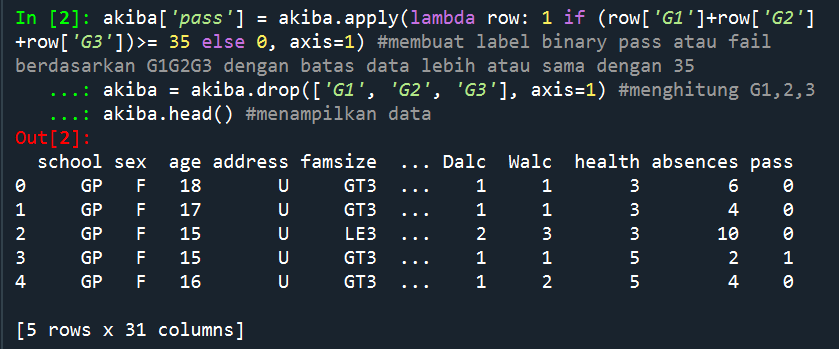
\includegraphics[width=12cm]{figures/chapter2/20.PNG}
    \caption{Nomor 2}
\end{figure}

\subsection{Nomor 3}

\begin{lstlisting}[language=Python]
#memanggil kolom pada file csv
akiba = pd.get_dummies(akiba, columns=['sex', 'school', 'address', 'famsize', 'Pstatus', 'Mjob',
                                       'Fjob', 'reason', 'guardian', 'schoolsup', 'famsup', 'paid',
                                       'activities', 'nursery', 'higher', 'internet', 'romantic'])
akiba.head() #menampilkan data
\end{lstlisting}

\par Hasilnya

\begin{figure}[H]
    \centering
    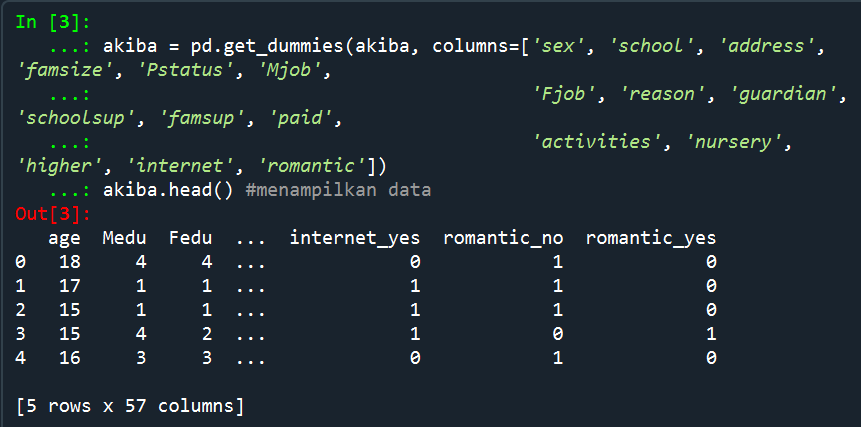
\includegraphics[width=12cm]{figures/chapter2/21.PNG}
    \caption{Nomor 3}
\end{figure}

\subsection{Nomor 4}

\begin{lstlisting}[language=Python]
akiba = akiba.sample(frac=1) #variable akiba dengan isi data sample
akiba_train = akiba[:500] #membagi data untuk training
akiba_test = akiba[500:] #membagi data untuk test

akiba_train_att = akiba_train.drop(['pass'], axis=1) #menghapus data yang telah lewat(pass) kemudian diinputkan
akiba_train_pass = akiba_train['pass'] #mengambil data pass saja

akiba_test_att = akiba_test.drop(['pass'], axis=1) #menghapus data yang telah lewat(pass) kemudian diinputkan
akiba_test_pass = akiba_test['pass'] #mengambil data pass saja

akiba_att = akiba.drop(['pass'], axis=1) #menghapus data yang telah lewat(pass) kemudian diinputkan
akiba_pass = akiba['pass'] #mengambil data pass saja

import numpy as np #import library numpy dengan alias np
print ("Passing: %a out of %a (%.2f%%)" % (np.sum(akiba_pass), len(akiba_pass), 100*float(np.sum(akiba_pass)) / len(akiba_pass))) #menampilkan data
\end{lstlisting}

\par Hasilnya

\begin{figure}[H]
    \centering
    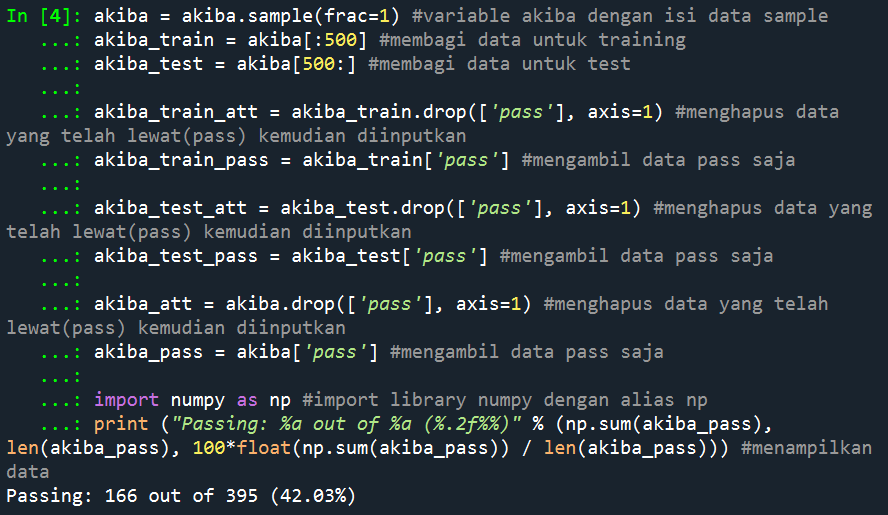
\includegraphics[width=12cm]{figures/chapter2/22.PNG}
    \caption{Nomor 4}
\end{figure}

\subsection{Nomor 5}

\begin{lstlisting}[language=Python]
from sklearn import tree #import library tree dari sklearn
tokyo = tree.DecisionTreeClassifier(criterion="entropy", max_depth=5) #membuat decision tree dengan max depth adalah 5
tokyo = tokyo.fit(akiba_train_att, akiba_train_pass) #memasukkan data untuk decision tree
\end{lstlisting}

\par Hasilnya

\begin{figure}[H]
    \centering
    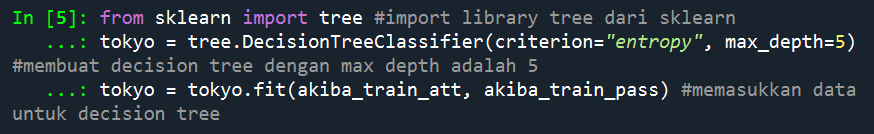
\includegraphics[width=12cm]{figures/chapter2/23.PNG}
    \caption{Nomor 5}
\end{figure}

\subsection{Nomor 6}

\begin{lstlisting}[language=Python]
import graphviz #import library graphviz
dot_data = tree.export_graphviz(tokyo, out_file=None, label="all", impurity=False, 
                                proportion=True, feature_names=list(akiba_train_att), 
                                class_names=["fail", "pass"], filled=True, rounded=True) #mendefinisikan data yang akan divisualisasikan di decision tree
graph = graphviz.Source(dot_data) #memasukkan data ke variable graph
graph #menampilkan gambar
\end{lstlisting}

\par Hasilnya

\begin{figure}[H]
    \centering
    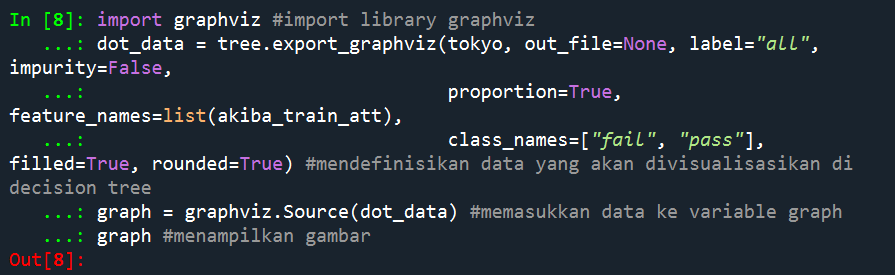
\includegraphics[width=12cm]{figures/chapter2/24.PNG}
    \caption{Nomor 6}
\end{figure}

\par visualisasi decision tree

\begin{figure}[H]
    \centering
    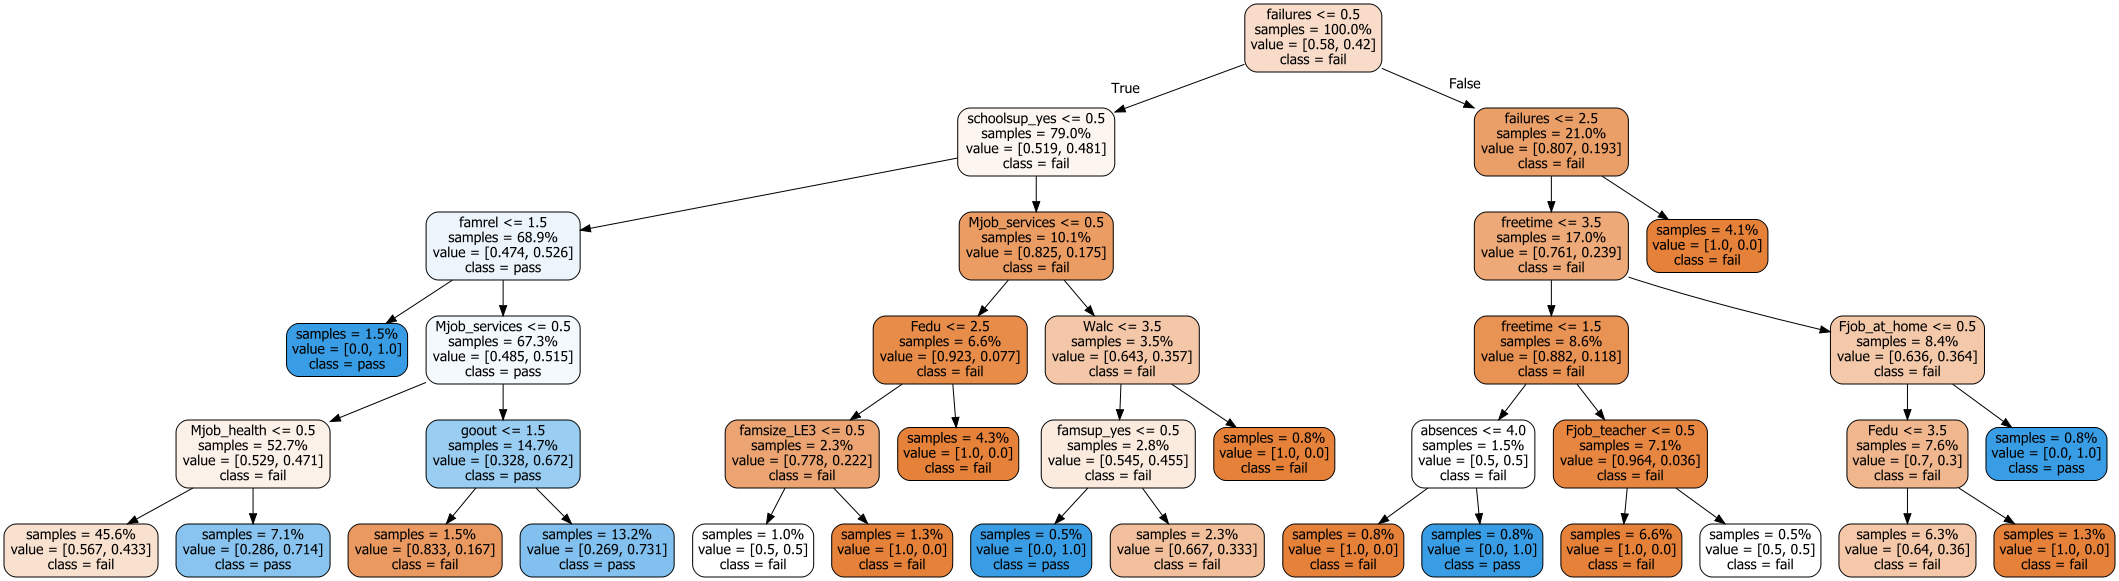
\includegraphics[width=12cm]{figures/chapter2/25.png}
    \caption{Nomor 6}
\end{figure}

\subsection{Nomor 7}

\begin{lstlisting}[language=Python]
tree.export_graphviz(tokyo, out_file="student-performance.dot",
                     label="all", impurity=False,
                     proportion=True,
                     feature_names=list(akiba_train_att),
                     class_names=["fail", "pass"],
                     filled=True, rounded=True) #untuk ekspor graph decision tree
\end{lstlisting}

\par Hasilnya

\begin{figure}[H]
    \centering
    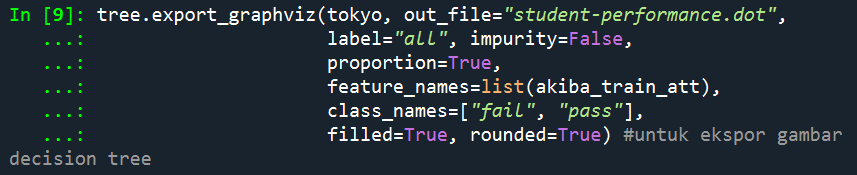
\includegraphics[width=12cm]{figures/chapter2/26.PNG}
    \caption{Nomor 7}
\end{figure}

\par Lokasi file student-performance.dot pada komputer, dapat diliat yang ditandai biru.

\begin{figure}[H]
    \centering
    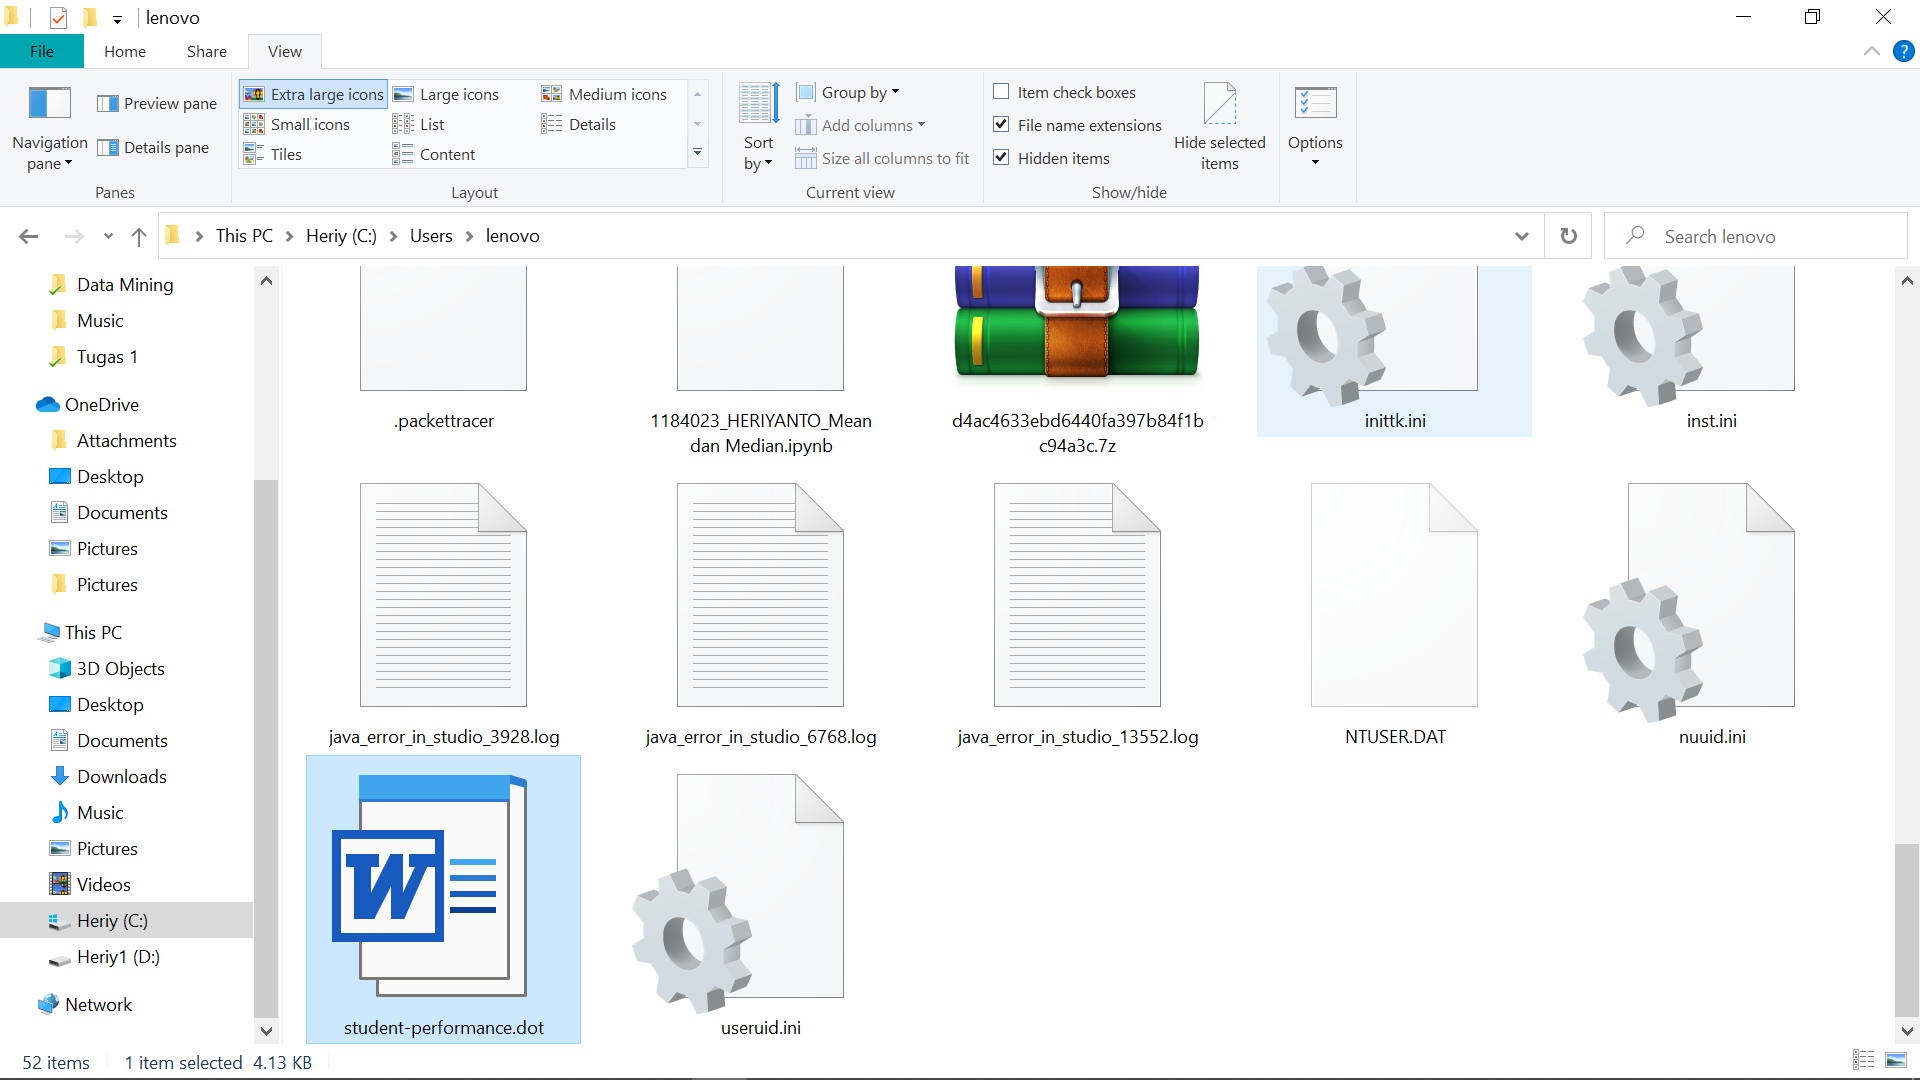
\includegraphics[width=12cm]{figures/chapter2/27.PNG}
    \caption{Nomor 7}
\end{figure}

\subsection{Nomor 8}

\begin{lstlisting}[language=Python]
tokyo.score(akiba_test_att, akiba_test_pass) #menghitung prediksi nilai yang akan datang
\end{lstlisting}

\par Hasilnya error, kenapa hasilnya error karena hasil prediksi dari student-mat.csv itu nol(0), jadi tidak menampilkan nilai prediksi. Untuk menampilkan nilai prediksi minimal nilainya harus 1.

\begin{figure}[H]
    \centering
    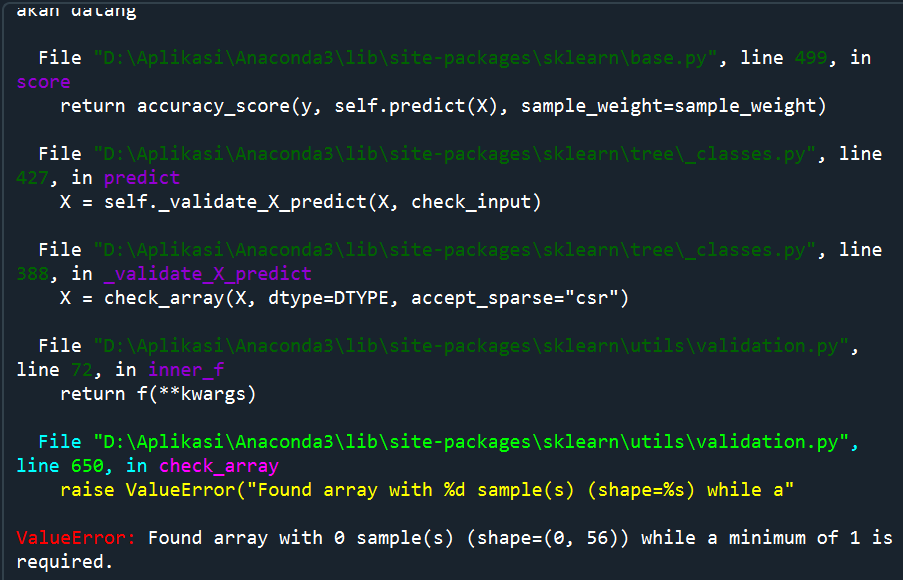
\includegraphics[width=12cm]{figures/chapter2/28.PNG}
    \caption{Nomor 8}
\end{figure}

\subsection{Nomor 9}

\begin{lstlisting}[language=Python]
from sklearn.model_selection import cross_val_score #import module cross_val_score dari sklearn.model_selection
okinawa = cross_val_score(tokyo, akiba_att, akiba_pass, cv=5) #pembagian data menjadi 5 bagian
print ("Accuracy: %0.2f (+/- %0.2f)" % (okinawa.mean(), okinawa.std() * 2)) #menampilkan hasil dari rata-rata dan standar deviasi dikali 2
\end{lstlisting}

\par Hasilnya

\begin{figure}[H]
    \centering
    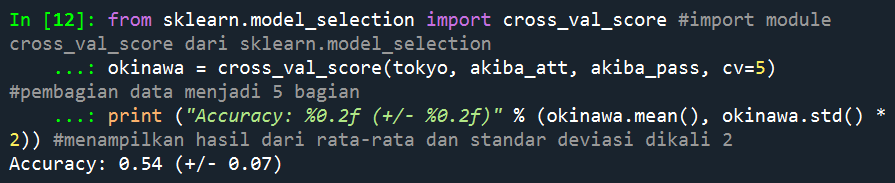
\includegraphics[width=12cm]{figures/chapter2/29.PNG}
    \caption{Nomor 9}
\end{figure}

\subsection{Nomor 10}

\begin{lstlisting}[language=Python]
for max_depth in range(1, 20): #pengulangan max depth dalam jangkauan 1-20
    tokyo = tree.DecisionTreeClassifier(criterion="entropy", max_depth=max_depth) #membuat decision tree 
    okinawa = cross_val_score(tokyo, akiba_att, akiba_pass, cv=5) #pembagian data menjadi 5 bagian
    print("Max depth: %d, Accuracy: %0.2f (+/- %0.2f)" % (max_depth, okinawa.mean(), okinawa.std() * 2)) #menampilkan hasil dari rata-rata dan standar deviasi dikali 2
\end{lstlisting}

\par Hasilnya

\begin{figure}[H]
    \centering
    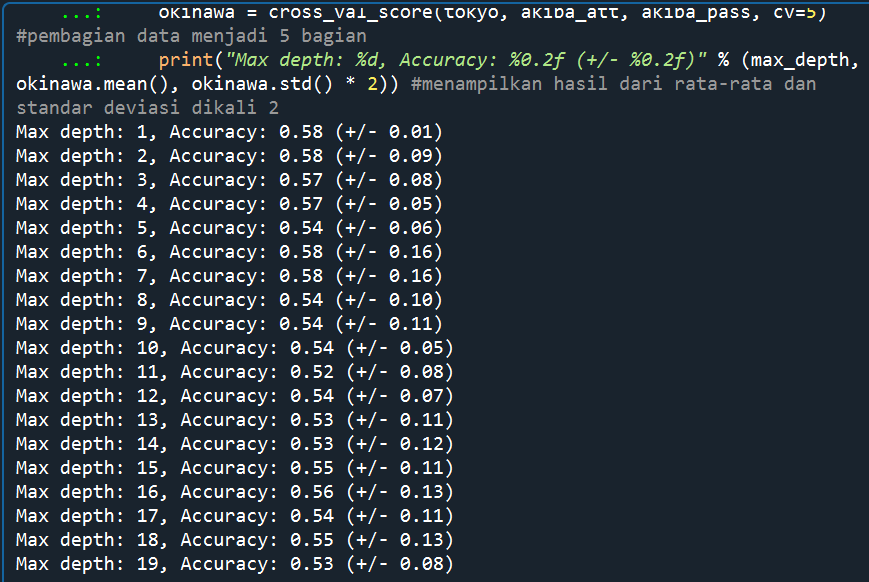
\includegraphics[width=12cm]{figures/chapter2/30.PNG}
    \caption{Nomor 10}
\end{figure}

\subsection{Nomor 11}

\begin{lstlisting}[language=Python]
depth_acc = np.empty((19,3), float) #membuat array baru
i = 0 #variable i dengan isi 0
for max_depth in range(1, 20): #pengulangan dalam jangkauan 1-20
    tokyo = tree.DecisionTreeClassifier(criterion="entropy", max_depth=max_depth) #membuat decision tree
    okinawa = cross_val_score(tokyo, akiba_att, akiba_pass, cv=5) #pembagian data menjadi 5 bagian 
    depth_acc[i,0] = max_depth #meng-inputkan data max depth ke array depth acc
    depth_acc[i,1] = okinawa.mean() #meng-inputkan rata-rata ke array depth acc 
    depth_acc[i,2] = okinawa.std() * 2 #meng-inputkan nilai standar deviasi ke array depth acc
    i += 1

depth_acc
\end{lstlisting}

\begin{figure}[H]
    \centering
    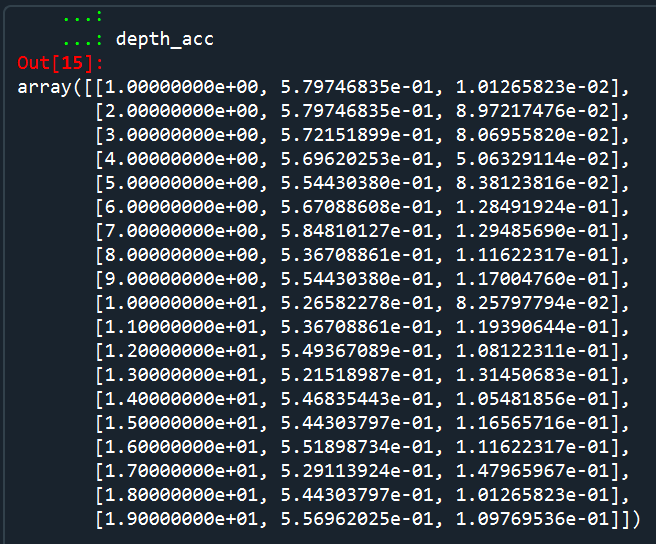
\includegraphics[width=12cm]{figures/chapter2/31.PNG}
    \caption{Nomor 11}
\end{figure}

\subsection{Nomor 12}

\begin{lstlisting}[language=Python]
import matplotlib.pyplot as plt #import library matplotlib dengan alias plt
fig, ax = plt.subplots() #membuat plot baru
ax.errorbar(depth_acc[:,0], depth_acc[:,1], yerr=depth_acc[:,2]) #mengisi data plot
plt.show() #menampilkan data plot
\end{lstlisting}

\begin{figure}[H]
    \centering
    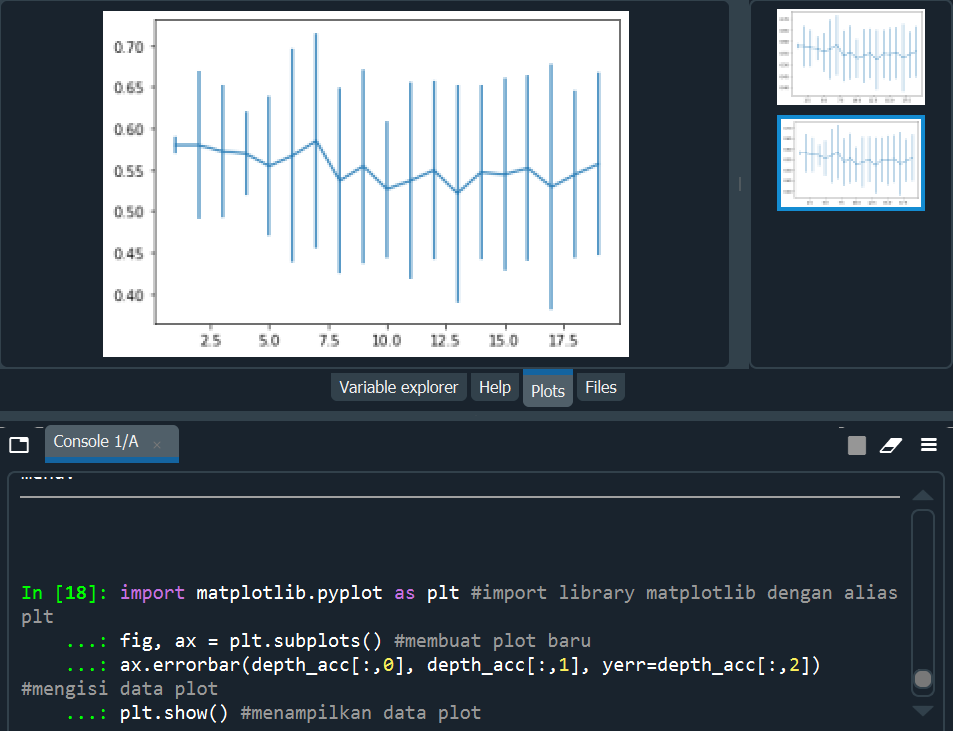
\includegraphics[width=12cm]{figures/chapter2/32.PNG}
    \caption{Nomor 12}
\end{figure}